\documentclass{beamer}
\usepackage{ctex}
\usepackage{graphicx}
\usepackage{tikz}
\usepackage{amsmath}
\usepackage{pgfplots}
\usepackage{pgfplotstable}
\usepackage{subcaption}
\usepackage{listings}

\lstset{
  language=Python, % 设置代码语言
  basicstyle=\small\ttfamily, % 设置代码基本样式
  keywordstyle=\color{blue}, % 设置关键字样式
  commentstyle=\color{green!40!black}, % 设置注释样式
  stringstyle=\color{orange}, % 设置字符串样式
  showstringspaces=false, % 不显示字符串中的空格
  breaklines=true, % 自动断行
  frame=single, % 代码框
}

\title{NFT 与 Web3 简介 \\ 以及 WHUpunk 的基本玩法}
\author{怀菁}
\institute{武汉大学}
\date{\today}

\usetheme{Madrid}

\begin{document}

\frame{\titlepage}

\begin{frame}
    \frametitle{我昨晚看到的一则新闻}

    \begin{columns}
        \begin{column}{0.5\textwidth}
            \centering
            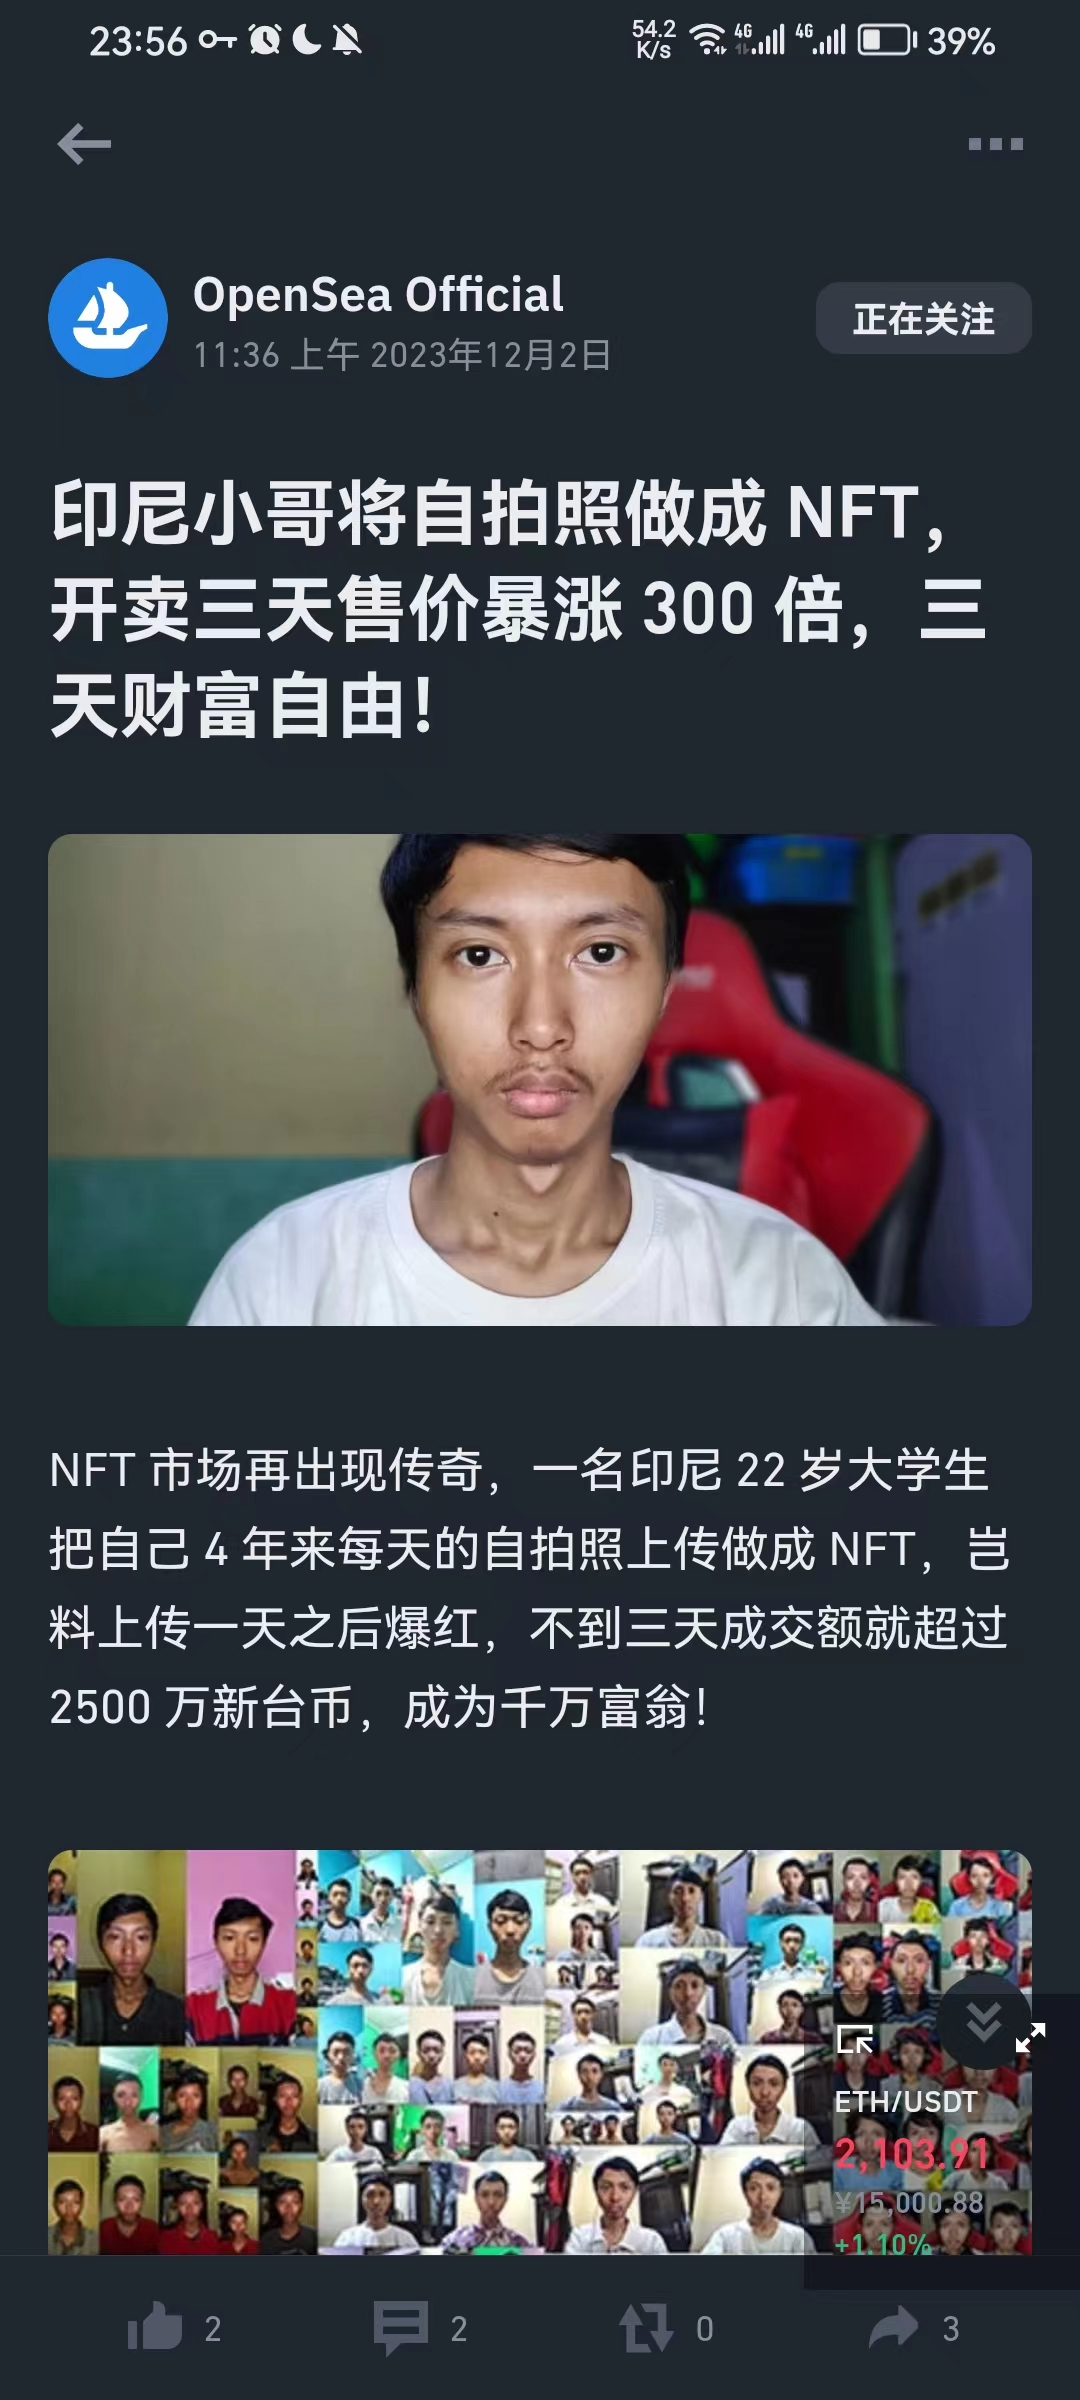
\includegraphics[width=0.8\textwidth]{p1.jpg}
        \end{column}
        \begin{column}{0.5\textwidth}
            \begin{figure}[htbp]
                \centering
                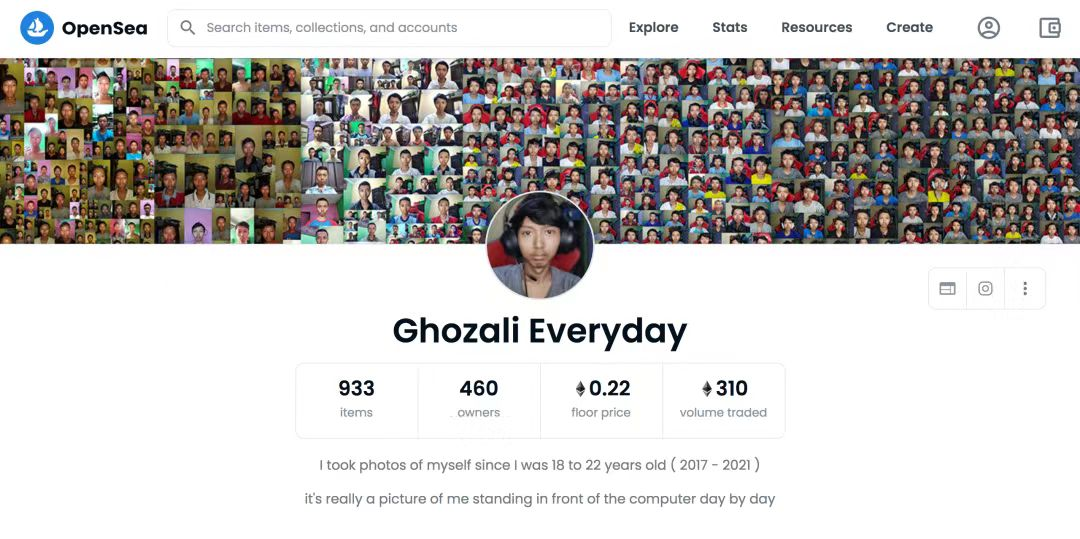
\includegraphics[width=\textwidth]{p3.jpg}
            \end{figure}
            \begin{figure}[htbp]
                \centering
                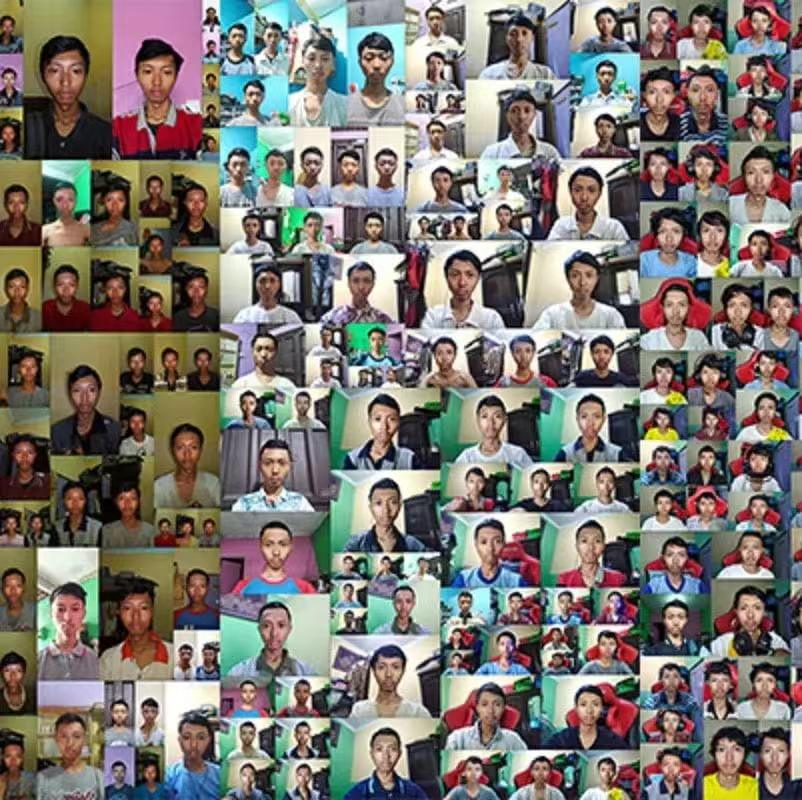
\includegraphics[width=0.8\textwidth]{p2.jpg}
            \end{figure}
        \end{column}
    \end{columns}
\end{frame}

\begin{frame}
    \frametitle{什么是 NFT}
    \begin{itemize}
        \item Non-Fungible Token:非同质化代币
        \item 同质化代币:例如美元、比特币、现货黄金等能够替换、具有统一性、可接近无穷拆分的代币。一张10美元总是能够换来十张1美元,美国矿工和中国矿工挖出来的比特币永远是一模一样的。
        \item 非同质化代币并不新鲜,成套的邮票、我们小时候玩的集卡,都是 NFT 的雏形。
    \end{itemize}
    \begin{columns}
        \begin{column}{0.5\textwidth}
            \begin{figure}[htbp]
                \centering
                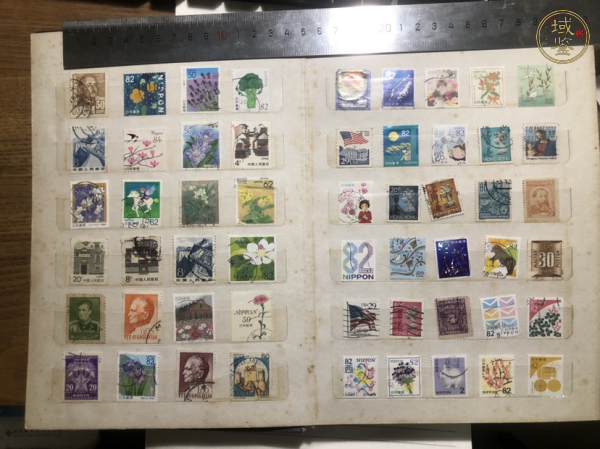
\includegraphics[width=0.9\textwidth]{p4.jpg}
            \end{figure}
        \end{column}
        \begin{column}{0.5\textwidth}
            \begin{figure}[htbp]
                \centering
                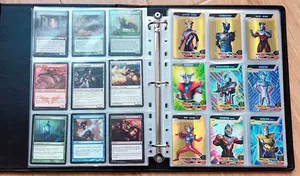
\includegraphics[width=0.9\textwidth]{p5.png}
            \end{figure}
        \end{column}
    \end{columns}
\end{frame}

\begin{frame}
    \frametitle{有代表性的 NFT 项目}
    \begin{columns}
        \begin{column}{0.33\textwidth}
            \centering
            CryptoPunk

            总市值 \$1,193,579,954

            地板价 \$119,430
            
\includegraphics[width=0.9\textwidth]{cryptopunk.jpg}
        \end{column}
        \begin{column}{0.33\textwidth}
            \centering
            Bored Ape

            总市值 \$618,711,286

            地板价 \$62,089
            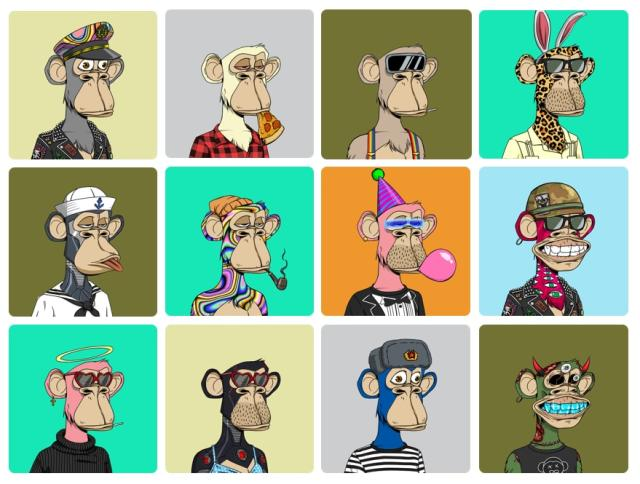
\includegraphics[width=\textwidth]{boredape.jpg}
        \end{column}
        \begin{column}{0.33\textwidth}
            \centering
            浙江大学 求是鹰 NFT
            国内项目 \ 不能炒作
            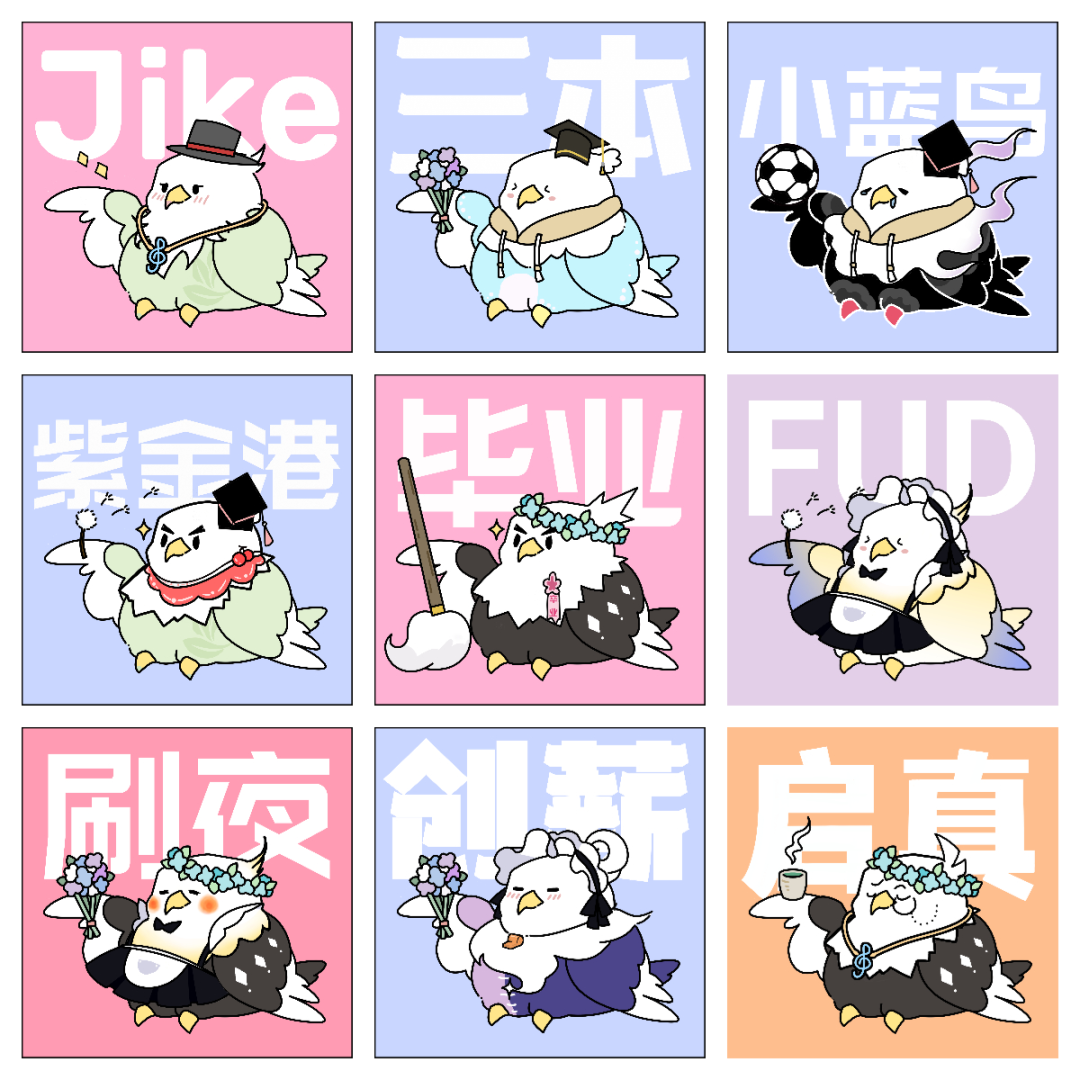
\includegraphics[width=0.9\textwidth]{qiushiying.png}
        \end{column}
    \end{columns}

\end{frame}

\begin{frame}
    \frametitle{NFT 的特点}

    \begin{itemize}
        \item 不可拆分
        \item 不可篡改
        \item 供给有限
        \item 独一无二
        \item 私有财产神圣不可侵犯
    \end{itemize}

    这些特点是如何兼顾的呢?
    
    要解释这个问题就不得不理解区块链的基本机制。
\end{frame}

\begin{frame}
    \frametitle{密码学基础:哈希函数}

    \begin{itemize}
        \item 又称散列函数,是一类函数的总称
        \item 按照维基百科的定义,哈希函数是一种从任何一种数据中创建小的数字“指纹”的方法
    \end{itemize}

    要想将一个只由小写字母组成的字符串 $S$ 映射为一个数字,一个可行的哈希算法是:

    $$H(S) = \sum_{i = 1}^n (S_i-\text{'a'})$$

    很显然,这样得出来的函数值并没有承载自变量的全部信息。用函数值倒推自变量的全部内容,是几乎是不可能的事情。可以认为哈希算法通常是对数据的“有损压缩”。
    
    但是,如果我们已知一个函数值,我们往往能根据对一系列可能的自变量快速地\textbf{检验}出每个自变量在哈希过后是否与给定的函数值相匹配,从而检验出这份数据的完整性和正确性。

\end{frame}

\begin{frame}
    \frametitle{区块链基本运行机制}

    请进入浏览器,访问 \url{https://blockchaindemo.org/}

\end{frame}

\begin{frame}[fragile]
    \frametitle{从简单转账到 NFT}

    \begin{itemize}
        \item 最开始的区块链(也就是比特币)只支持简单转账
        \item 但是真实的经济生活中,人们的经济活动往往非常复杂,涉及到触发条件、交易流程、权益分配等问题
        \item 人们希望将这些内容写成代码,编译为可执行程序,然后在区块链上执行这些程序
        
    \end{itemize}

    \begin{lstlisting}
        if time >= 2023-12-01:
            MyAccount.balance += 10
            YourAccount.balance -= 10
    \end{lstlisting}
  
    \begin{itemize}
        \item 这就是智能合约(Smart Contract)。你可以认为“公共账本”升级为了“公共电脑”,而智能合约就在一台所有人参与建设、参与监管并认可其真实性的公共电脑上运行。
        \item NFT 的铸造、转移、买卖、销毁、收益分配都是由智能合约实现
        \item ERC-721 协议规定了一个 NFT 应当具有的基本功能,以太坊上 NFT 项目的开发人员都会选择遵守这份标准
    \end{itemize}

\end{frame}

\begin{frame}
    \frametitle{ERC-721 标准简介}

    ERC-721 标准倡议,一个 NFT 合约应当具备以下功能:

    \begin{itemize}
        \item 可以转移,即具有 transferFrom() 函数
        \item 可以授权,即具有 approve() 函数
        \item 可以查询某个 NFT 的主人,即具有 ownerOf() 函数
        \item 可以查询某地址持有该系列 NFT 的数量,即具有 balanceOf() 函数
    \end{itemize}

    在实际开发中,我们还约定俗成地实现以下功能:

    \begin{itemize}
        \item tokenURI() :用于查询某个 NFT 的详细信息,包括图片内容等
        \item mint() :用于铸造一个新的 NFT 
    \end{itemize}

\end{frame}

\begin{frame}
    \frametitle{Burnt Banksy 烧画卖 NFT}

    画作原本价值:不到\$ 100,000

    烧毁后铸造 NFT 卖出价值:\$ 380,000

    \begin{figure}[htbp]
        \centering
        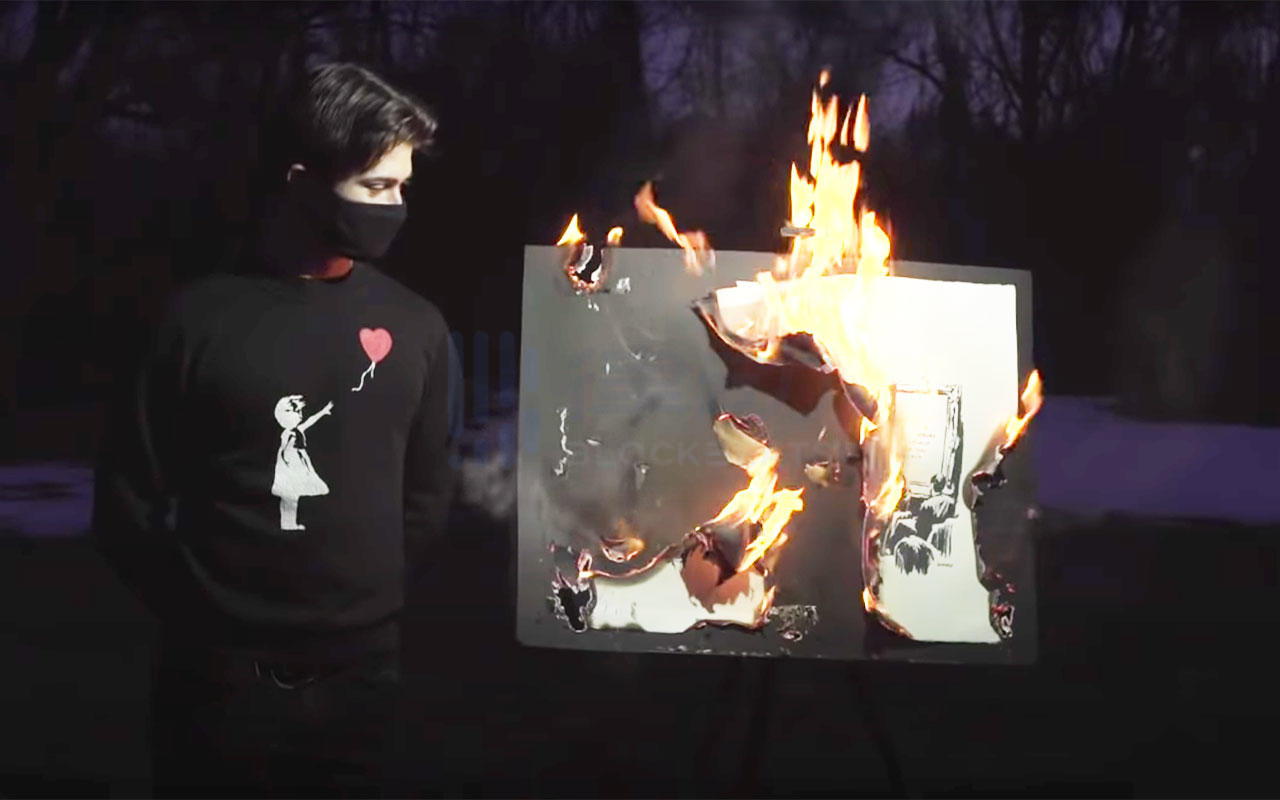
\includegraphics[width=0.8\textwidth]{burn.png}
    \end{figure}

\end{frame}

\begin{frame}
    \frametitle{区块链能用来干什么?}

    \begin{itemize}
        \item 利用不可篡改性
            \begin{itemize}
                \item 发布新闻,方便翻合订本打脸
                \item 人人参与记录历史,让历史不再是任凭统治者打扮的小姑娘
                \item 记录言论,防止删号跑路
                \item 发布个人内容,可以永久保存
                \item 明确产权
            \end{itemize}
        \item 利用去中心化
            \begin{itemize}
                \item 反抗金融霸权,让每个人都能参与金融活动及其规则制定
                \item 反抗文化霸权,抗内容审查,实现真正的创作自由
                \item 将社会契约写成智能合约,让每个人享有更真实的民主权利
            \end{itemize}
        \item 利用透明性
            \begin{itemize}
                \item 促进信息流通,构建完全竞争市场
                \item 监督企业财务状况,监控大鳄资金流向
                \item 反洗钱
                \item 生成基于共识的真实信息
            \end{itemize}
        \item 利用匿名性
            \begin{itemize}
                \item 保护个人隐私,防止经济活动中造成个人信息泄露
            \end{itemize}
        \item 你想用它什么它就能干什么……
    \end{itemize}

\end{frame}

\begin{frame}
    \frametitle{Web3到底是什么?}

    目前一个比较通行的说法是, Web3 是根据区块链网络构建起来的新一代互联网。

    \begin{itemize}
        \item 基础设施:公链、扩容、云服务
        \item 去中心化金融 DeFi:DEX、Lending、Liquid Staking、稳定币、衍生品、RWA、钱包
        \item 非同质化代币 NFT
        \item 去中心化自治组织 DAO
        \item 链游 GameFi
        \item 创造者经济 Creator Economics
        \item 社交媒体 SocialFi
    \end{itemize}

\end{frame}

\begin{frame}
    \frametitle{Web3需要用到的知识}

    \begin{itemize}
        \item 数学:代数、密码学、信息论
        \item 计算机科学:合约开发、网络安全、数据结构、分布式系统、前端
        \item 经济学:经济学理论、金融工程、博弈论、项目生态治理、营销
        \item 设计学与美学
        \item 人文科学:历史、哲学、社会学、政治学
        \item 法学
        \item 心理学
        \item 硬件相关:通信、电子、物理、化学
        \item 传播学
        \item 环境学
        \item ……
    \end{itemize}

    Web3是全人类迄今为止所有智慧的结晶,任何知识都将助力Web3的建设,都在Web3领域有用武之地。

\end{frame}

\begin{frame}
    \frametitle{MetaMask 的介绍及安装}

    MetaMask 是一个去中心化的开源区块链钱包,可以作为浏览器插件,使用起来非常方便。它是我们与区块链交互的窗口之一。

    \begin{enumerate}
        \item 准备好翻墙软件
        \item 打开浏览器
        \item 访问 \url{https://metamask.io/}
        \item 点击 Download 并安装,如果你的浏览器是 Edge 或 Chrome ,网页会跳转到扩展商店,安装扩展程序到浏览器即可
        \item 现在在你浏览器的右上角应该出现了一个小狐狸图标
    \end{enumerate}

\end{frame}

\begin{frame}
    \frametitle{开始创建钱包之前}

    一个钱包有四个要素:

    \begin{itemize}
        \item 公钥:也就是钱包的地址,是公开信息,有人向你转账时,他必须知道你的地址才能转账。
        \item 私钥:也就是钱包的密码。公钥是用私钥按照特定算法生成的。\textbf{注意:任何时候都不能把私钥泄露给任何人!}任何人获取了私钥之后,就能够提取其中全部的资金!诈骗犯提款的时候不需要向区块链证明自己的真实身份!区块链只认私钥,不认人!\textbf{且资金丢失永远无法找回!}
        \item 助记词:因为私钥是很长一串字符串,所以需要一个助记词来记住它。实际上,私钥就是用助记词生成的出来的。\textbf{泄露助记词就必然泄露私钥!任何时候都不可以向任何人泄露自己助记词!}一套助记词一般有 12 个英文单词,导入钱包时\textbf{缺一不可!}\textbf{一旦你遗忘助记词,那么你的资金永远无法找回!}
        \item 密码:仅用于在这一台设备上登录钱包。其他设备上无效!只有助记词可以跨设备登录钱包\textbf{无法找回!}
    \end{itemize}

    \textbf{没有人能够帮你找回你的私钥助记词!将它写下来、刻在金属上,或保存在多个秘密位置,这样就不会丢失。如果丢失了,它就会永远消失。}

\end{frame}

\begin{frame}
    \frametitle{创建钱包流程}
    警告:\textbf{永远不要向任何人泄露私钥和助记词!}

    \textbf{务必保管好自己的助记词!完整抄下来!存多个备份在不同的位置!}

    \

    \begin{columns}
        \begin{column}{0.4\textwidth}
            1. 点击浏览器扩展程序中的 MetaMask
            \begin{figure}[htbp]
                \centering
                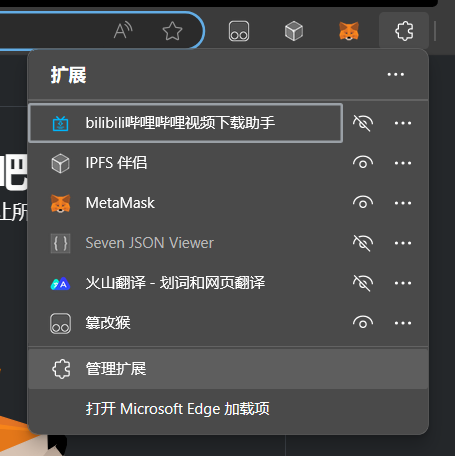
\includegraphics[width=\textwidth]{m1.png}
            \end{figure}
        \end{column}
        \begin{column}{0.5\textwidth} 
            2. 如果你没有创建过钱包,那么就点击创建新钱包

            如果你曾经创建过钱包,那么点击导入钱包
            \begin{figure}[htbp]
                \centering
                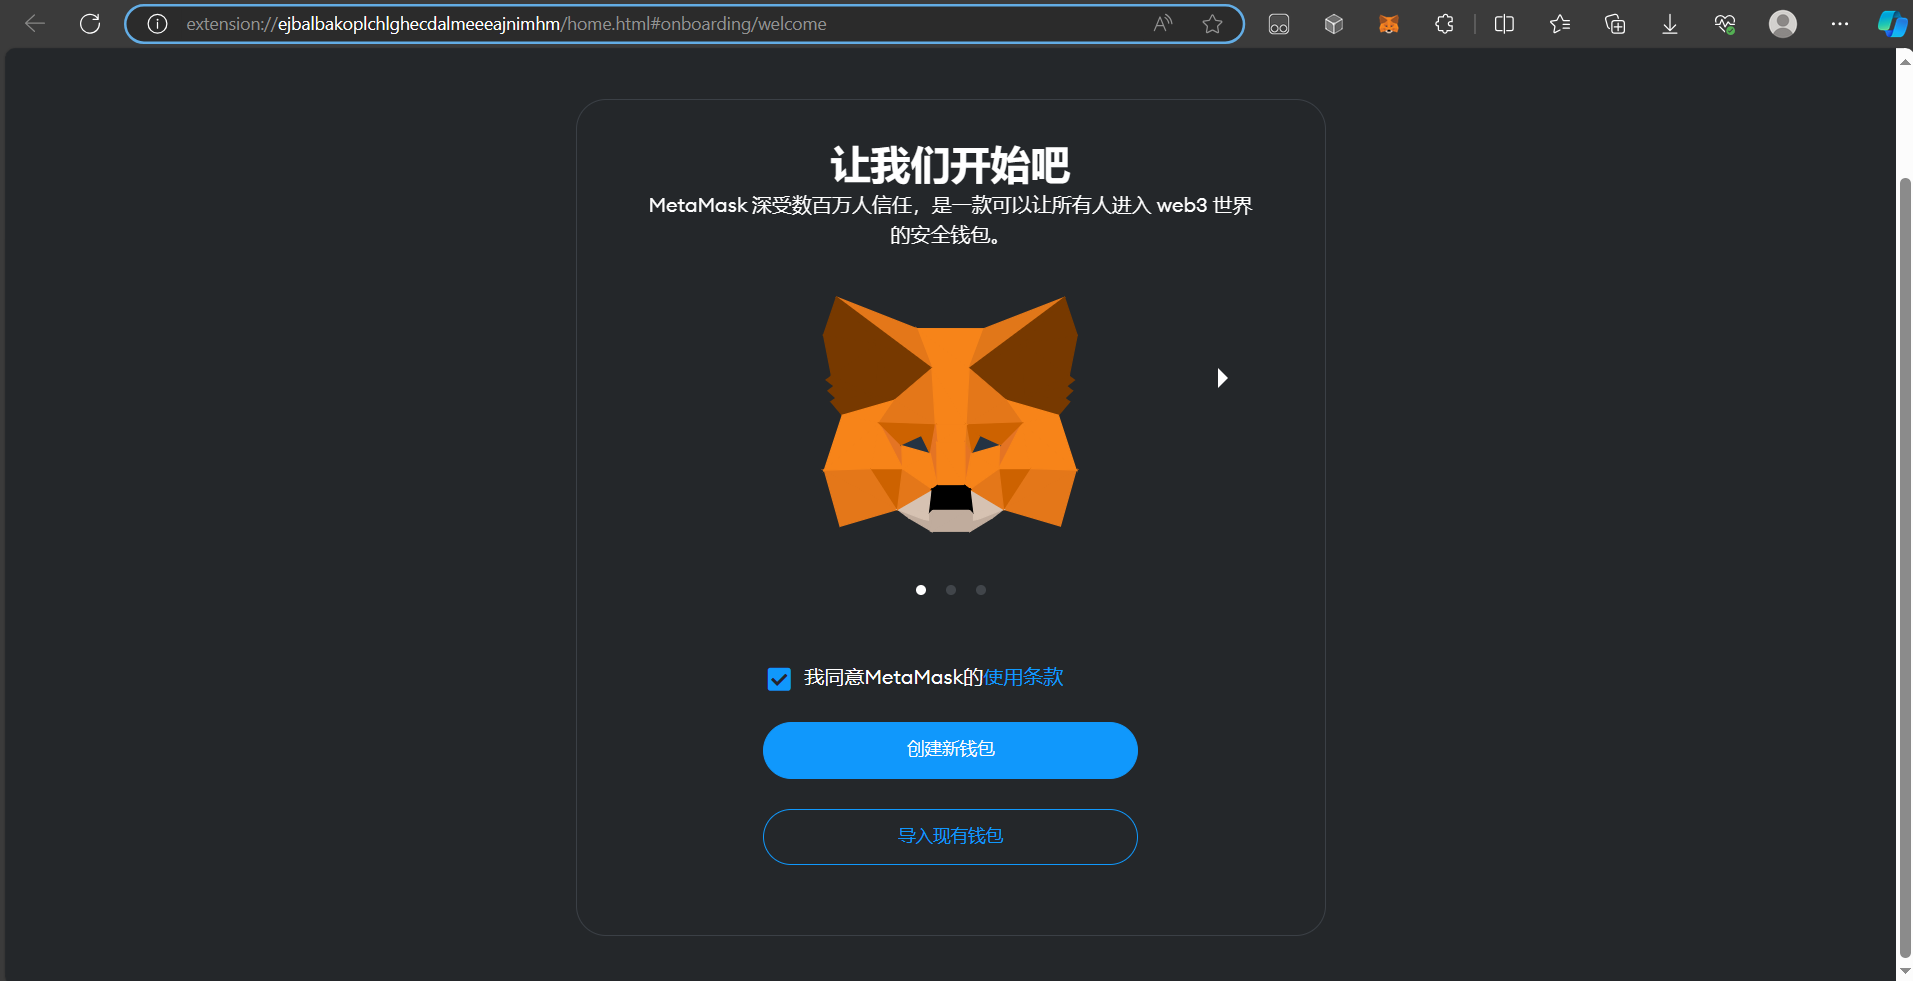
\includegraphics[width=\textwidth]{m2.png}
            \end{figure}
        \end{column}
    \end{columns}

\end{frame}

\begin{frame}
    \frametitle{创建钱包流程}

    警告:\textbf{永远不要向任何人泄露私钥和助记词!}

    \textbf{务必保管好自己的助记词!完整抄下来!存多个备份在不同的位置!}

    \

    3. 逐字逐句仔细阅读 MetaMask 的安全警示,务必理解所有内容

    \begin{figure}[htbp]
        \centering
        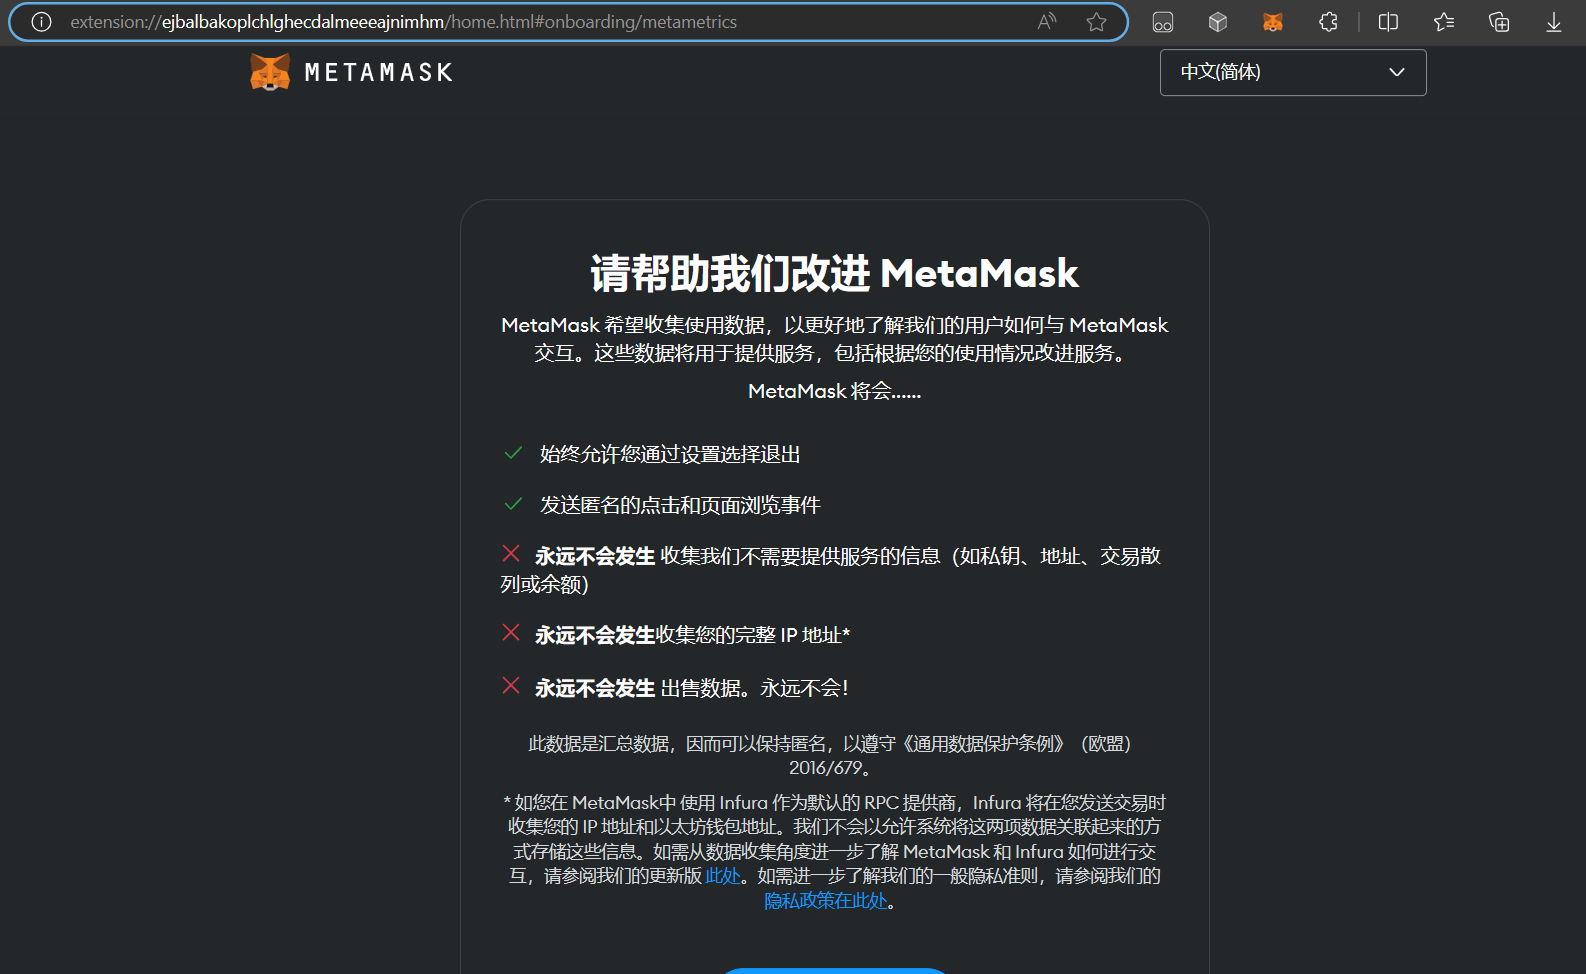
\includegraphics[width=0.9\textwidth]{m3.png}
    \end{figure}

\end{frame}

\begin{frame}
    \frametitle{创建钱包流程}

    警告:\textbf{永远不要向任何人泄露私钥和助记词!}

    \textbf{务必保管好自己的助记词!完整抄下来!存多个备份在不同的位置!}

    \

    4. 设置本机登录密码。此密码\textbf{不可找回!}在其他设备无效!\textbf{有了密码也必须牢记助记词!}

    \begin{figure}[htbp]
        \centering
        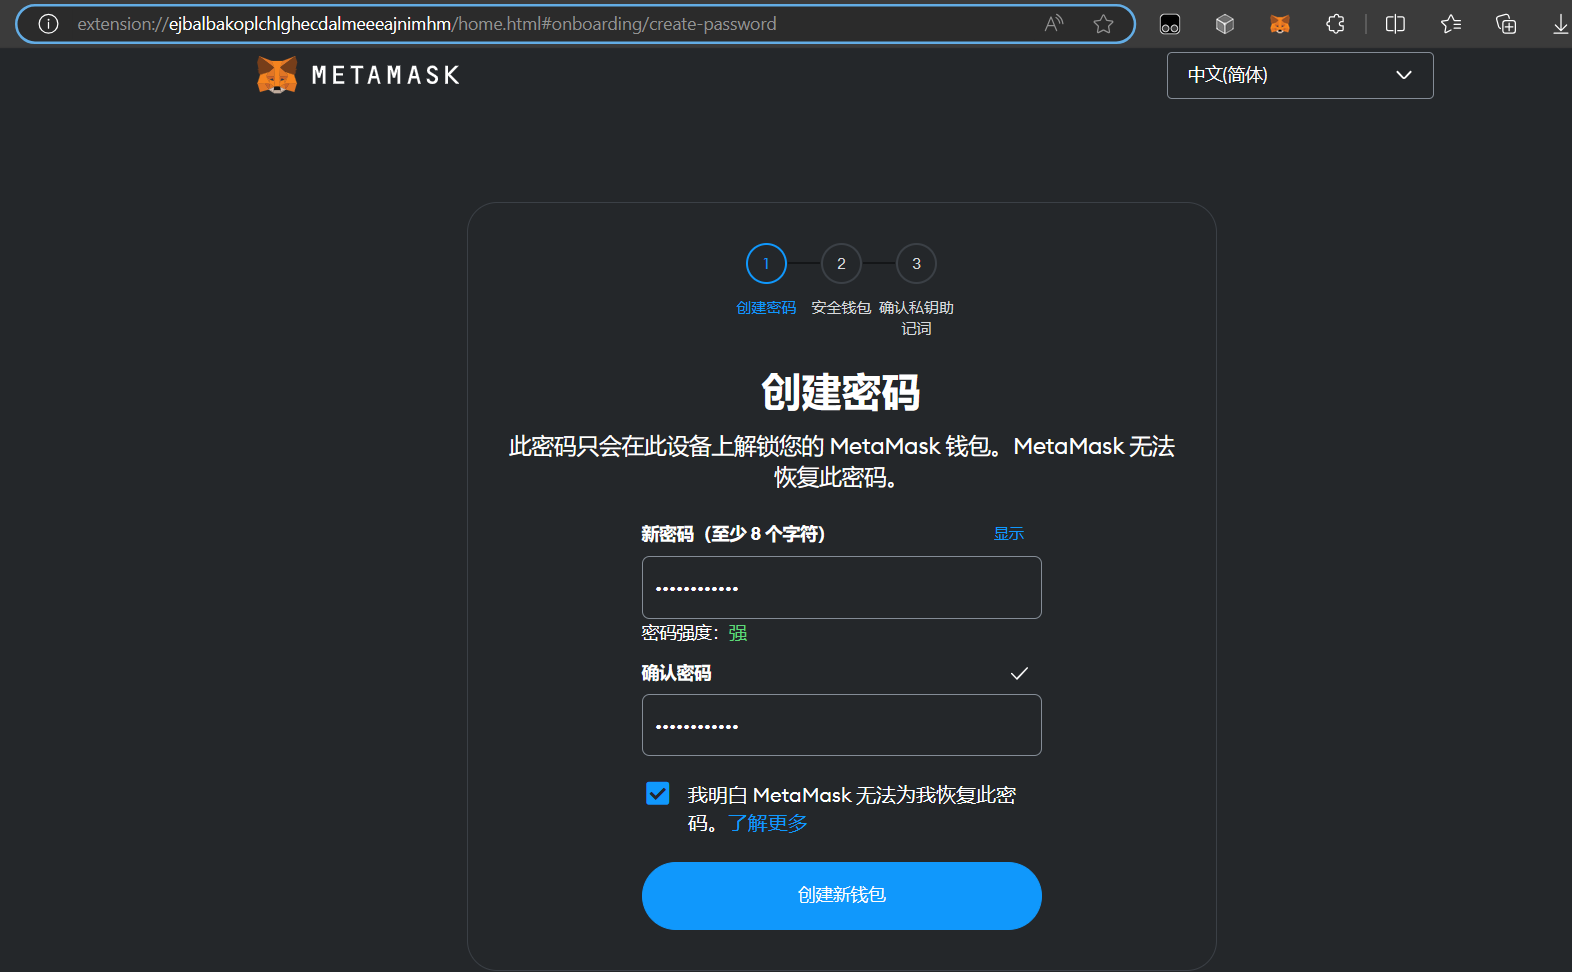
\includegraphics[width=0.8\textwidth]{m4.png}
    \end{figure}

\end{frame}

\begin{frame}
    \frametitle{创建钱包流程}

    警告:\textbf{永远不要向任何人泄露私钥和助记词!}

    \textbf{务必保管好自己的助记词!完整抄下来!存多个备份在不同的位置!}

    \

    5. 认真观看视频

    \begin{figure}[htbp]
        \centering
        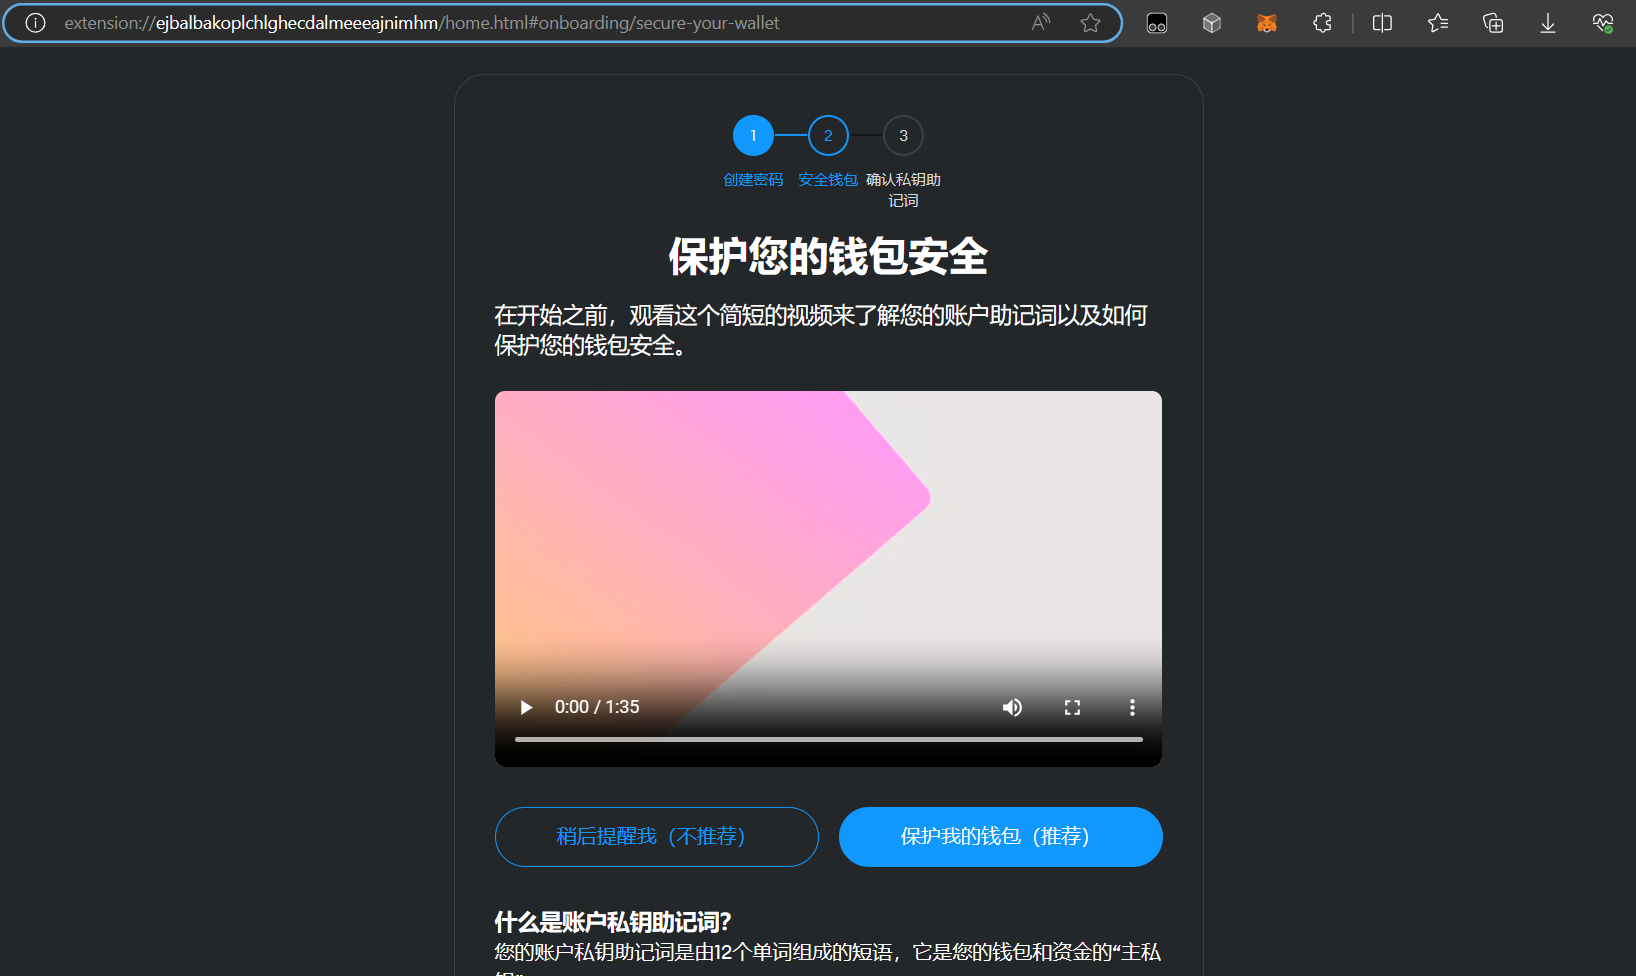
\includegraphics[width=0.8\textwidth]{m5.png}
    \end{figure}

\end{frame}

\begin{frame}
    \frametitle{创建钱包流程}

    警告:\textbf{永远不要向任何人泄露私钥和助记词!}

    \textbf{务必保管好自己的助记词!完整抄下来!存多个备份在不同的位置!}

    \


    \begin{columns}
        \begin{column}{0.5\textwidth}
            6. 准备好纸和笔,确保周围没有人在看你的屏幕,点击“显示私钥助记词”,并抄下助记词,确保每一个字母都是对的,顺序也是对的。\textbf{任何微小的错误都会导致资金全部丢失!}

            \
            
            \
            
            \

            \

            \
        \end{column}
        \begin{column}{0.5\textwidth}
            \begin{figure}
                \centering
                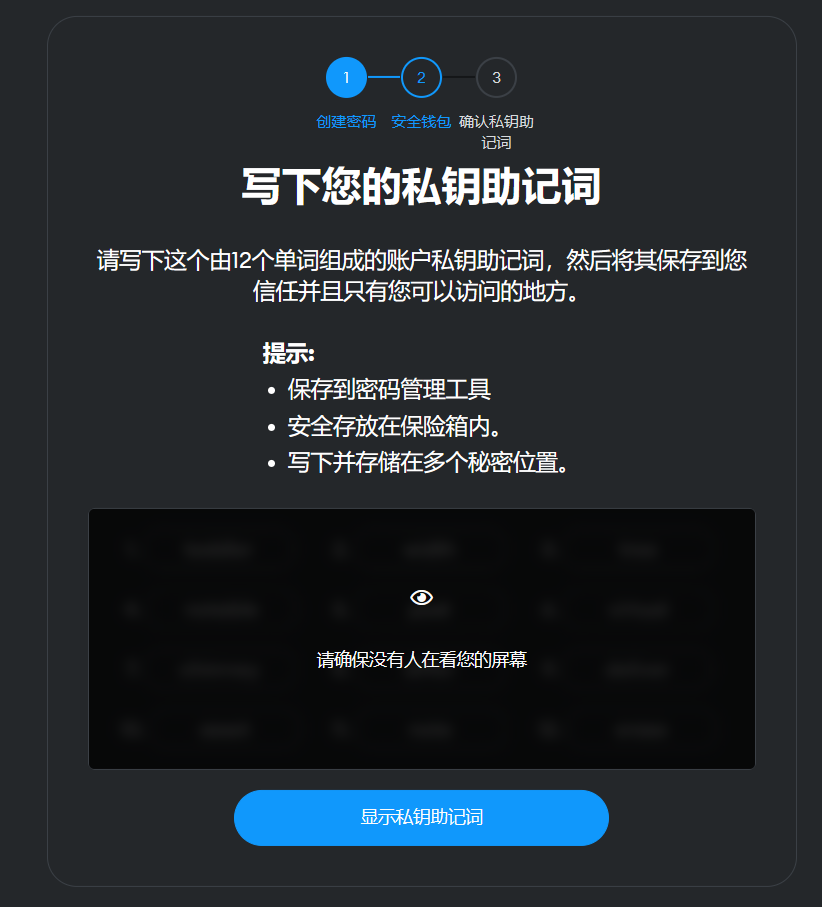
\includegraphics[width=\textwidth]{m6.png}
            \end{figure}
        \end{column}
    \end{columns}

\end{frame}

\begin{frame}
    \frametitle{创建钱包流程}

    警告:\textbf{永远不要向任何人泄露私钥和助记词!}

    \textbf{务必保管好自己的助记词!完整抄下来!存多个备份在不同的位置!}

    \

    7. 根据纸上抄的助记词,补全电脑上的助记词,并点击确认

    如果你抄错了助记词,可以点击浏览器左上角退回之前的页面重抄

    \begin{figure}
        \centering
        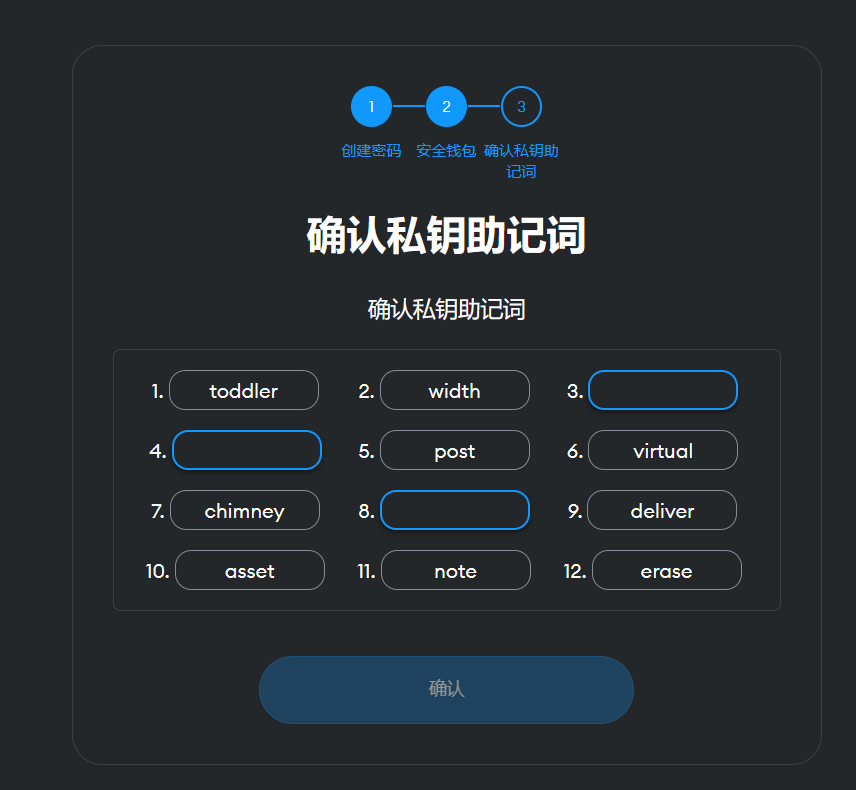
\includegraphics[width=0.5\textwidth]{m7.png}
    \end{figure}

\end{frame}

\begin{frame}
    \frametitle{创建钱包流程}

    警告:\textbf{永远不要向任何人泄露私钥和助记词!}

    \textbf{务必保管好自己的助记词!完整抄下来!存多个备份在不同的位置!}

    \

    8. 钱包创建完成。如果你刚刚记录私钥助记词的时候是用脑子记的,而没有手抄下来的,请倒回去抄下来!

    如果你需要重温助记词,可以在设置-安全与隐私-显示私钥助记词中再次看到自己的助记词。这样的操作不建议做太多次,因为你的电脑屏幕随时都有可能被监控。

    \begin{figure}
        \centering
        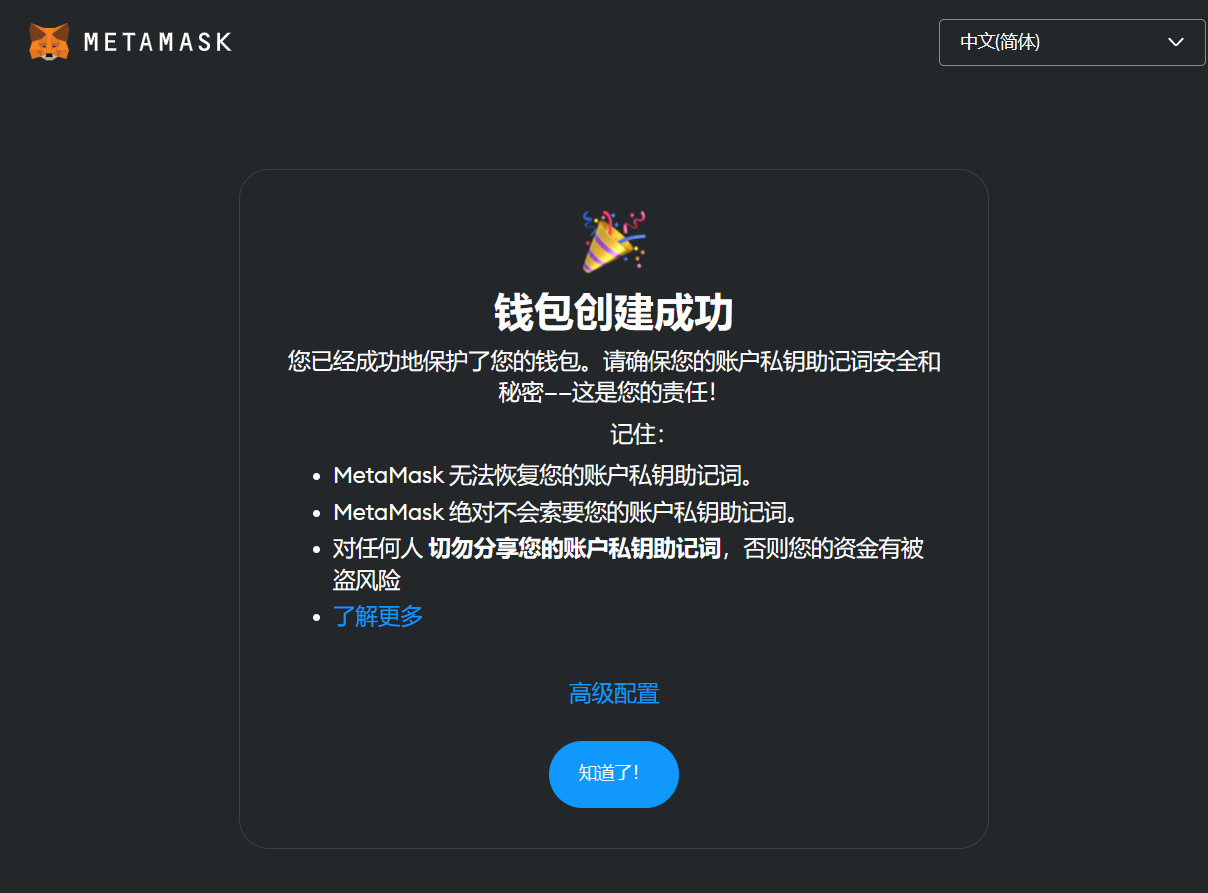
\includegraphics[width=0.5\textwidth]{m8.png}
    \end{figure}

\end{frame}

\begin{frame}
    \frametitle{熟悉钱包界面}

    

    \begin{columns}
        \begin{column}{0.55\textwidth}
            回到浏览器,点击 MetaMask ,会弹出一个小窗。你与区块链的大多数操作都可以在这里完成。

            单击切换网络-显示测试网络-Sepolia,就可以切换到 Sepolia 测试网。

            本次活动的大多数合约部署在 Sepolia 测试网上。测试网的钱都不是真金白银。但这并不意味着你就可以在安全问题上有所松懈,因为测试网和主网的地址、私钥都是一模一样的,只是所在的区块链网络不同。测试网的私钥泄露必然等同于主网私钥泄露。
        \end{column}

        \begin{column}{0.45\textwidth}
            \begin{figure}[t]
                \centering
                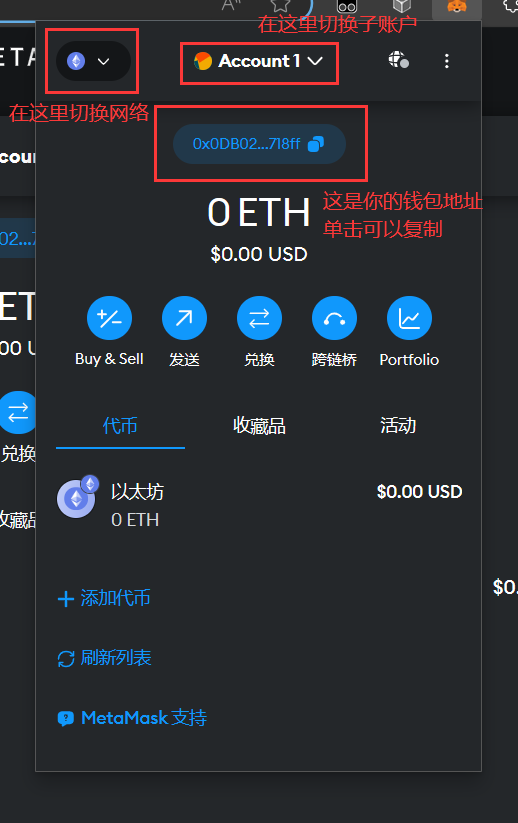
\includegraphics[width=\textwidth]{s1.png}
            \end{figure}
        \end{column}
    \end{columns}

\end{frame}

\begin{frame}
    \frametitle{领取测试网 SepoliaETH}

    \begin{enumerate}
        \item 访问 \url{https://sepoliafaucet.com/} ,这是 Alchemy 为我们提供的水龙头
        \item 用谷歌账号登录
        \item 复制钱包地址并粘贴到文本框中
        \item 完成人机身份验证
        \item 点击 “Send Me ETH” 并稍等片刻,0.5 个以太坊就会发送到你的钱包
    \end{enumerate}

\end{frame}

\begin{frame}
    \frametitle{相关合约地址}

    本次活动用到的测试网合约地址主要包括:

    \begin{itemize}
        \item DailyCheckIn: 0x3B1DF21A13f94b7B20566CE249a2E4a8E38E79d1
        \item CardEngine: 0xC455bc4f18719563421082206d53bB93933B4480
        \item Card: 0xb6240854CB4B410B9A92A6bdB7759B8E08270998
    \end{itemize}

    打开 \url{https://sepolia.etherscan.io/} ,这是一个区块浏览器,可以用来查看交易、地址与合约。
    
    你可以搜索上面三个合约地址,就能看到合约的详细信息。
    
    你也可以搜索自己的钱包地址,你会看到有一笔资金转入。这就是刚刚水龙头转给你的 ETH 。

\end{frame}

\begin{frame}
    \frametitle{签到合约交互}

    两次签到的时间间隔不能小于 6 小时,否则交易会回滚,签到必然失败。

    在浏览器中搜索 DailyCheckIn 合约,并点击 Contract 。

    \begin{figure}
        \centering
        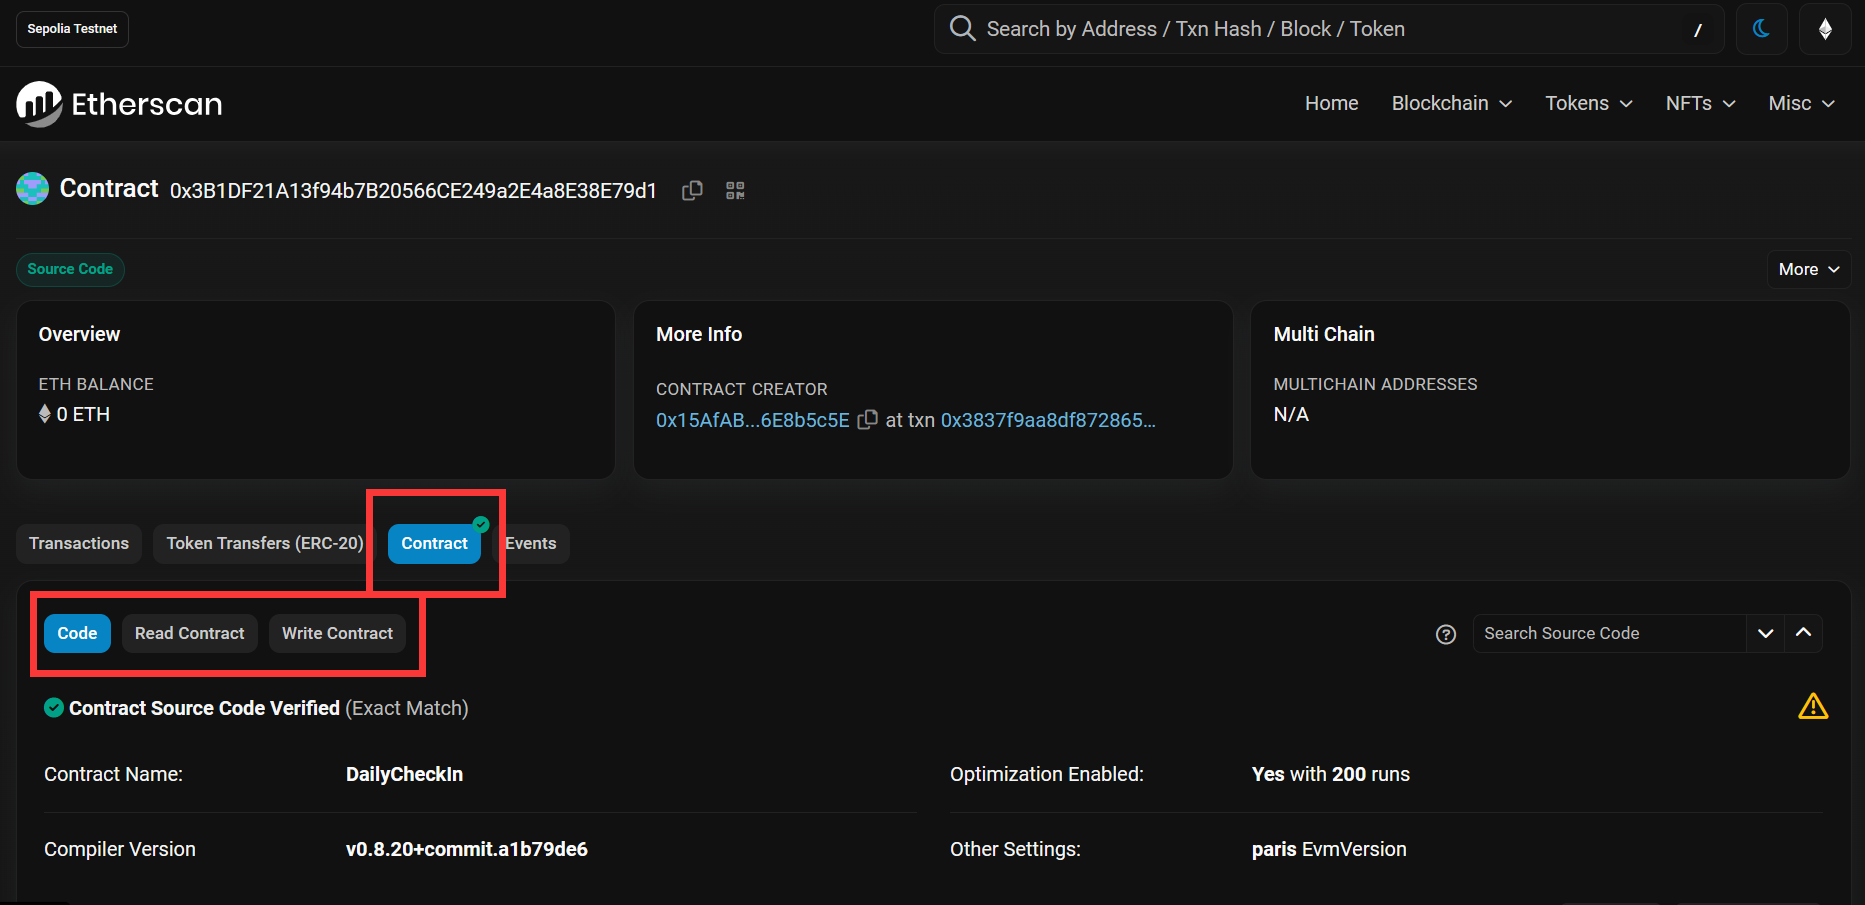
\includegraphics[width=0.8\textwidth]{s2.png}
    \end{figure}

    下面有三个选项卡:

    \begin{itemize}
        \item Code :你可以在这里看到合约的源代码
        \item Read Contract :用于读取合约的信息,通常不需要 gas fee
        \item Write Contract:用于写入并改变合约中的信息,需要付出 gas fee
    \end{itemize}

\end{frame}

\begin{frame}
    \frametitle{签到合约交互}

    \begin{columns}
        \begin{column}{0.6\textwidth}
            来到 Read Contract 。

            这里有两个函数:getCheckInTimesWithAddress() 和 getLastCheckInTimestampWithAddress() ,分别可以查询某一个地址成功签到的次数和最后一次签到的时间。

            \

            将你的钱包地址输入进去,点击 Query ,你会发现两个函数都返回了 0 。这是因为你从来没有成功签到过。
        \end{column}

        \begin{column}{0.4\textwidth}
            \begin{figure}
                \centering
                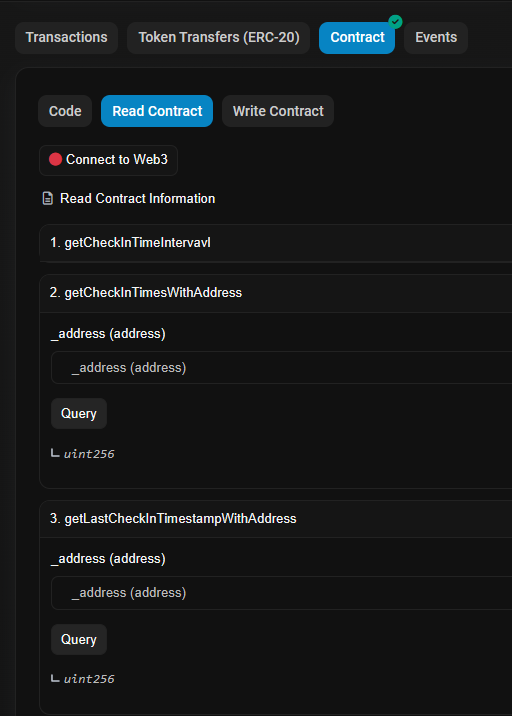
\includegraphics[width=\textwidth]{s7.png}
            \end{figure}
        \end{column}
    \end{columns}

\end{frame}

\begin{frame}
    \frametitle{签到合约交互}

    进入 Write Contract ,这里有 3 个函数,但其实只有第一个 CheckIn 是有用的。后面两个只有 Owner 有调用权限,且与核心功能无关。

    为了与合约交互,Etherscan 需要与你的钱包连接起来。点击 Connect to Web3 ,并在弹出的窗口中确认连接。这些操作不需要 gas fee ,也不用转账。

    \begin{columns}
        \begin{column}{0.6\textwidth}
            \begin{figure}
                \centering
                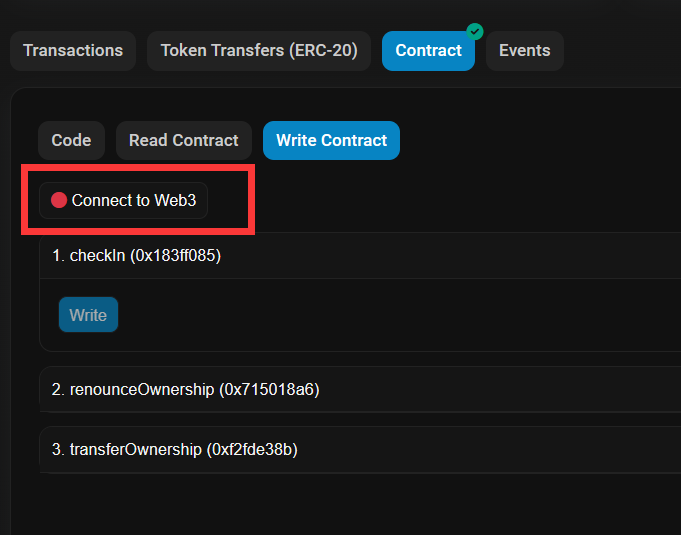
\includegraphics[width=\textwidth]{s3.png}
            \end{figure}
        \end{column}
        \begin{column}{0.25\textwidth}
            \begin{figure}
                \centering
                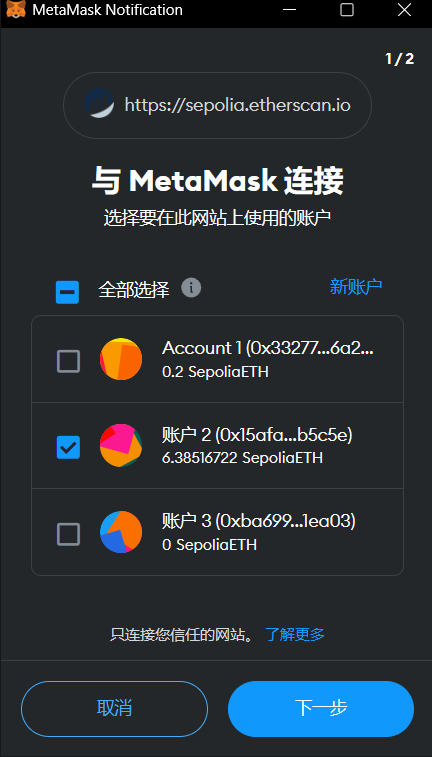
\includegraphics[width=\textwidth]{s4.png}
            \end{figure}
        \end{column}
    \end{columns}

\end{frame}

\begin{frame}
    \frametitle{签到合约交互}

    回到 Etherscan ,你会发现它已经和你的钱包连接在一起了。

    点击 Write 签到。调用这个函数不用传入任何参数,你的钱包地址会自动被当做签到主体。这样设计能有效防止代签到。

    此时,MetaMask 将会弹出,需要你确认发送交易。签到的操作将会被记录在区块链上,因此需要消耗 gas fee 。由于这里的钱都是假钱,没必要心疼,直接确认即可。

    \begin{columns}
        \begin{column}{0.5\textwidth}
            \begin{figure}[htbp]
                \centering
                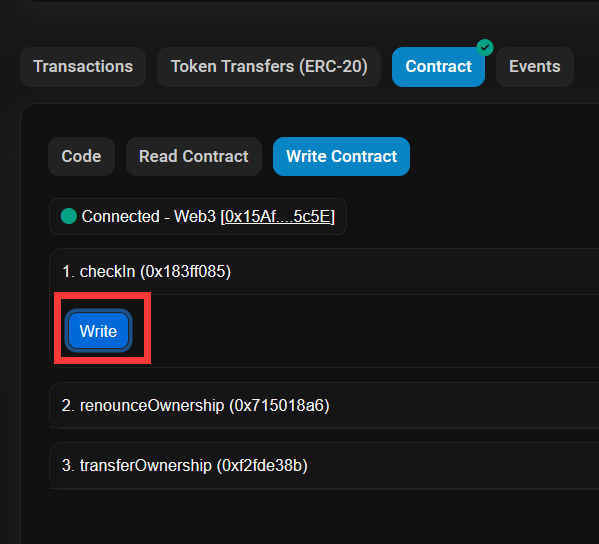
\includegraphics[width=0.9\textwidth]{s5.png}
            \end{figure}
        \end{column}
        \begin{column}{0.25\textwidth}
            \begin{figure}[htbp]
                \centering
                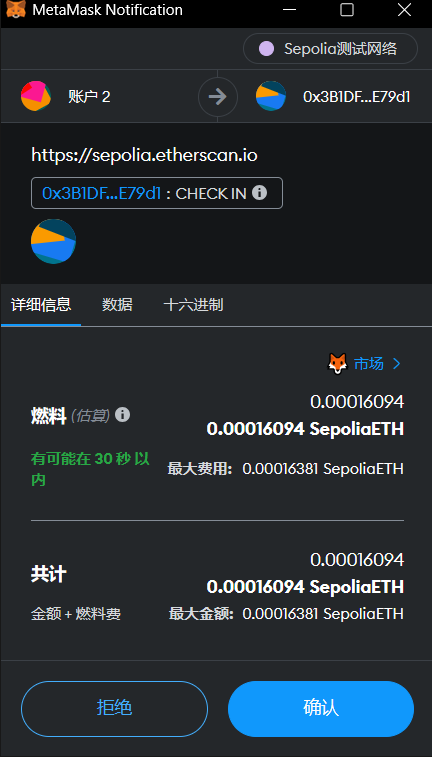
\includegraphics[width=0.9\textwidth]{s6.png}
            \end{figure}
        \end{column}
    \end{columns}

    
\end{frame}

\begin{frame}
    \frametitle{签到合约交互}

    \begin{columns}
        \begin{column}{0.6\textwidth}
            回到 Read Contract 。

            将你的钱包地址输入进去,点击 Query 你会发现你的签到次数变成了 1 ,上次签到的时间是一长串数字,这其实是你签到时刻的 Unix 时间戳。

            你也可以在上方的 Events 中看到所有参与者的签到记录。每次有人成功签到,合约就会释放一个 event 留作证据。

            \

            恭喜你!现在你已经掌握了签到合约的交互技能!世界上只有不到千万分之一的人能够将智能合约学到这个程度。
        \end{column}

        \begin{column}{0.4\textwidth}
            \begin{figure}
                \centering
                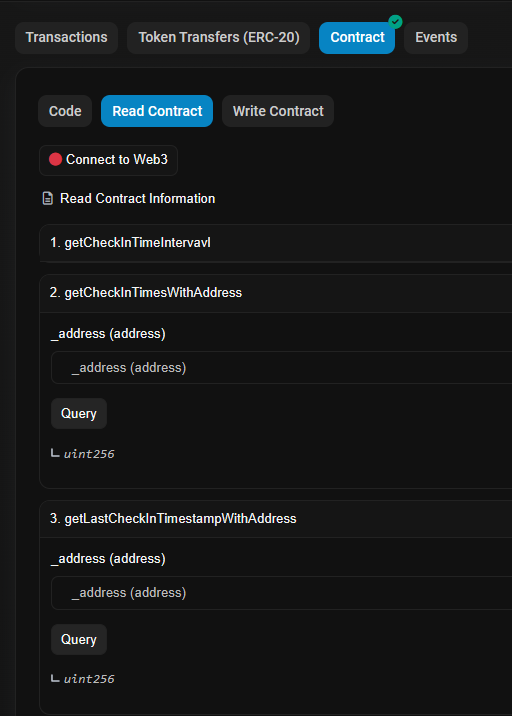
\includegraphics[width=\textwidth]{s7.png}
            \end{figure}
        \end{column}
    \end{columns}

\end{frame}

\begin{frame}
    \frametitle{集卡合约的交互}

    不过多赘述,先让大家自己探索一下。

    提示:先在 CardEngine 调用 draw 抽奖,等待至少两分钟后,调用 mint 铸造,并回到 MetaMask 用 Card 的地址与你的 tokenId 导入 NFT 。

\end{frame}

\begin{frame}
    \frametitle{模拟领取 NFT}

    

\end{frame}

\end{document}